\documentclass[xcolor=table, xcolor=dvipsnames]{beamer}
\usepackage[T1]{fontenc}
\usepackage{amsmath}
\usepackage[utf8]{inputenc}
\usepackage{anysize}
\usepackage{graphicx}
\usepackage{wasysym}
\usepackage{xcolor}
\usepackage{hyperref}


\usetheme[secheder]{Boadilla}
\begin{document}
\setbeamertemplate{navigation symbols}{}

%\renewcommand{\inserttotalframenumber}{11} 



\title[CLAS12: Run Group A]{Trigger Studies for $\eta' \rightarrow e^+e^-\gamma$}
    \author[]{Michael C. Kunkel / Daniel R. Lersch / James Ritman} 
      \date{$21.09.2017$} 
  %  \logo{\includegraphics[width=1cm]{}}
    \institute[IKP1 - Juelich]
    
    \begin{frame}
      \titlepage
    \end{frame}
 
  \begin{frame}
    \frametitle{Overview}
    \footnotesize
    
    %***********************************************************************************************************
    \begin{itemize}
      \item Trigger proposed for the upcoming CLAS12 spring run (20 days):
      \begin{itemize}
        \footnotesize
        \item[i)] NPHE(HTCC) $ > 5 ... 10$
        \item[ii)] $\Delta E(\text{PCAL + ECAL}) \ge 150\,\rm{MeV}$
      \end{itemize}
      \item This configuration would suppress $e^-$ with: $p \lesssim 0.7\,\rm{GeV/c}$ \\ {\color{blue}{$\Rightarrow$ Implemented in the actual CLAS12 PID-algorithm}} \\ {\color{blue}{$\Rightarrow$ We can do better than that}}
      \item Idea: 
      \begin{itemize}
        \footnotesize
        \item Momenta of dilepton-pair are predominantly distributed such that: \\ one low momentum lepton + one high momentum positron
        \item Look at p$(e^+)$ vs $p(e^-)$ for different cuts on both lepton momenta (corresponding to the trigger)\\  {\color{red}{$\Rightarrow$ Determine ratio of rejected / accepted events}}
        \item Also look at NPHE(LTCC), NPHE(HTCC) and $\Delta E(\text{PCAL + ECAL})$ for those different momentum cuts
      \end{itemize}
      \item Look at different torus-settings: $-100\%$ and $-75\%$, Solenoid: $60\%$
      \end{itemize}
      \end{frame}
      %***********************************************************************************************************
      
      
      %***********************************************************************************************************
      \begin{frame}
        \frametitle{$p(e^+)$ vs. $p(e^-)$ for Torus: $-100\%$ || $-75\%$ and Solenoid: $60\%$}
        \framesubtitle{reaction $ep\to p e' e^+ e^- \gamma$ was simulated $e^\pm$ PID based on TOF }
        \footnotesize
        \begin{figure}
          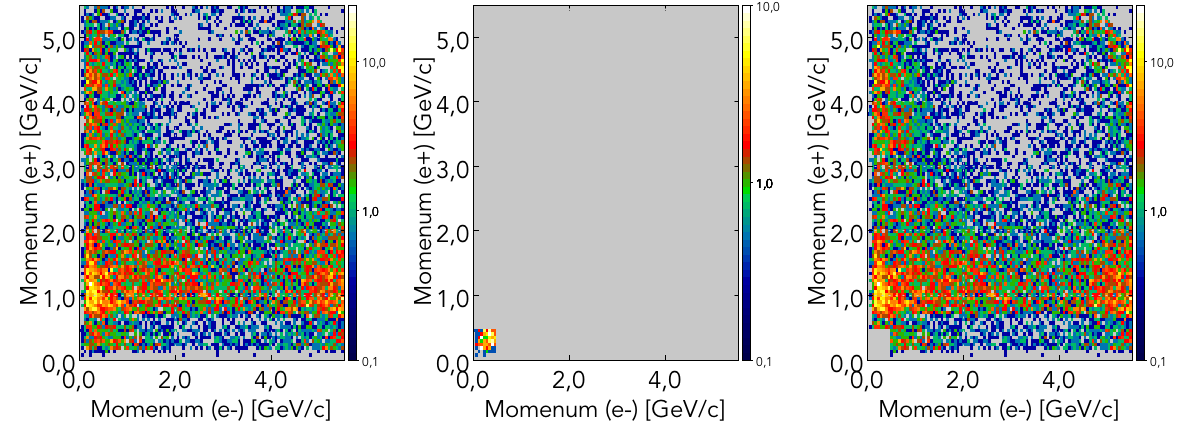
\includegraphics[width=1.0\textwidth,height=0.2\textwidth]{triggerStudies_Tor1_cut05_pEP_vs_pEM.png}\\
           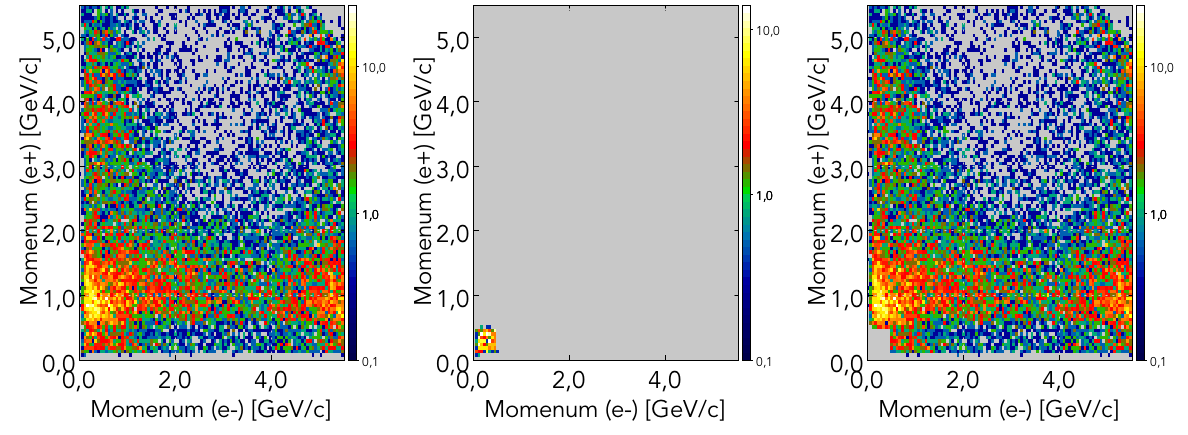
\includegraphics[width=1.0\textwidth,height=0.2\textwidth]{triggerStudies_Tor075_cut05_pEP_vs_pEM.png}
        \end{figure}
        
        \begin{itemize}
          \item Left: not cut 
          \item Centre: $p(e^+) \le 0.5\,\rm{GeV/c}$ and $p(e^-) \le 0.5\,\rm{GeV/c}$ 
          \item  Right: !($p(e^+) \le 0.5\,\rm{GeV/c}$ and $p(e^-) \le 0.5\,\rm{GeV/c}$)
          \item Top: Torus: $-100\%$ / Bottom: $-75\%$
        \end{itemize}
\end{frame}

\begin{frame}
        \frametitle{$p(e^+)$ vs. $p(e^-)$ for Torus: $-100\%$ || $-75\%$ and Solenoid: $60\%$}
	\footnotesize
        \begin{figure}
          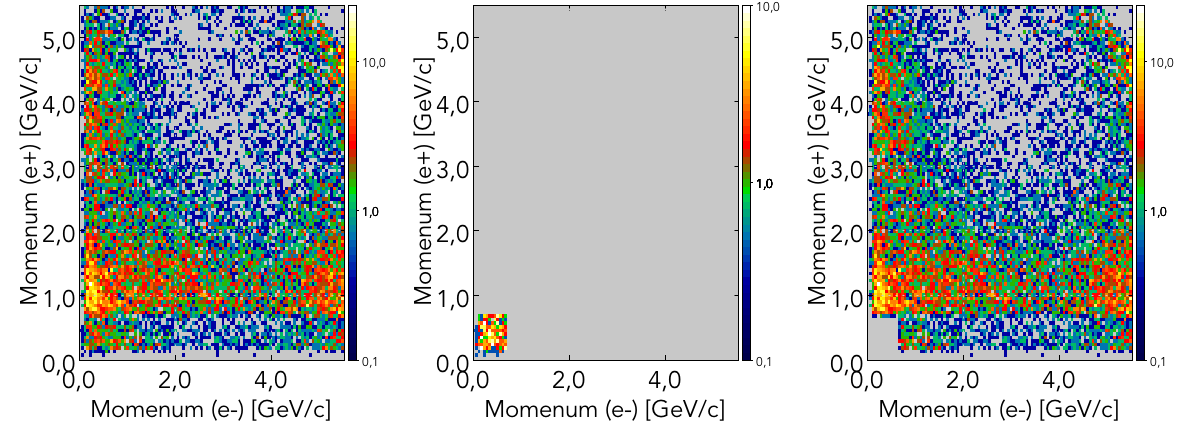
\includegraphics[width=1.0\textwidth,height=0.2\textwidth]{triggerStudies_Tor1_cut07_pEP_vs_pEM.png}\\
           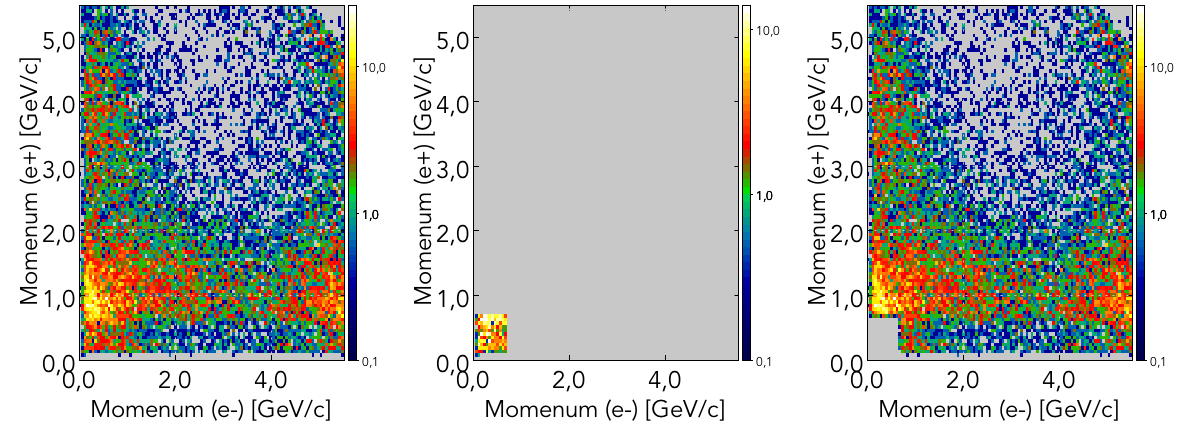
\includegraphics[width=1.0\textwidth,height=0.2\textwidth]{triggerStudies_Tor075_cut07_pEP_vs_pEM.png}
        \end{figure}
        
        \begin{itemize}
          \item Left: not cut 
          \item Centre: $p(e^+) \le 0.7\,\rm{GeV/c}$ and $p(e^-) \le 0.7\,\rm{GeV/c}$ 
          \item  Right: !($p(e^+) \le 0.7\,\rm{GeV/c}$ and $p(e^-) \le 0.7\,\rm{GeV/c}$)
          \item Top: Torus: $-100\%$ / Bottom: $-75\%$
        \end{itemize}
      \end{frame}
      %***********************************************************************************************************
      
      
      %***********************************************************************************************************
      \begin{frame}
        \frametitle{LTCC and HTCC vs. Momentum}
        \footnotesize
          \framesubtitle{No cut on $p(e^+)$ and $p(e^-)$}
           
           \begin{figure}
             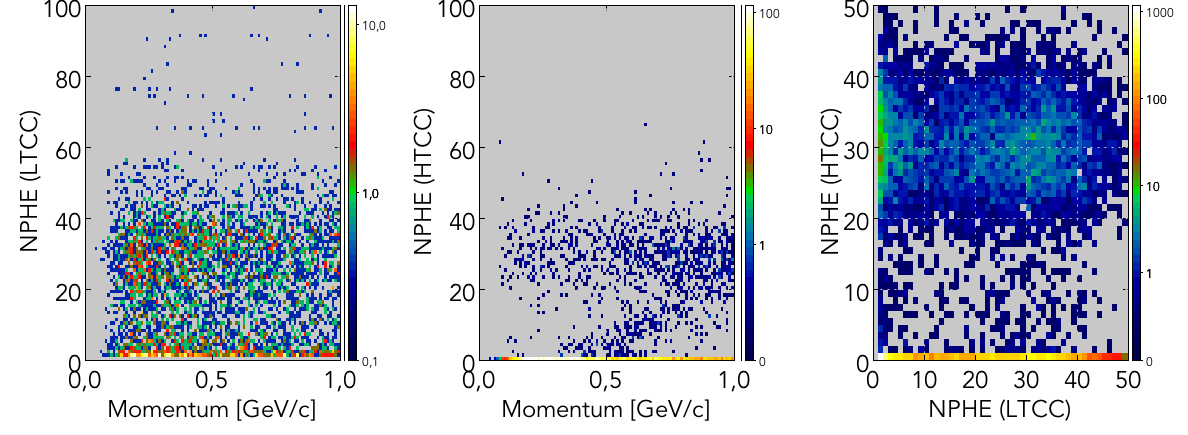
\includegraphics[width=1\textwidth,height=0.25\textwidth]{triggerStudies_Tor1_LTCC_HTCC_P.png}\\
             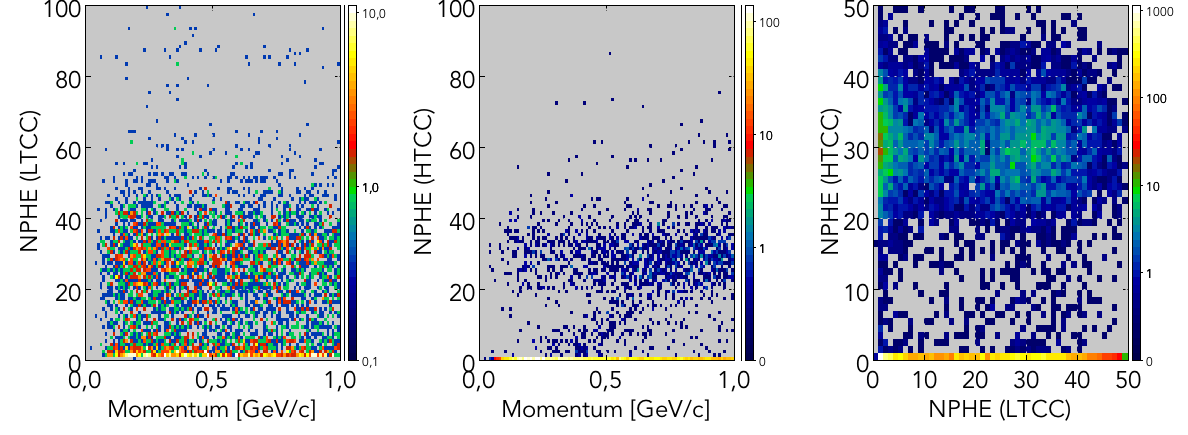
\includegraphics[width=1\textwidth,height=0.25\textwidth]{triggerStudies_Tor075_cut05_LTCC_HTCC_P.png}
           \end{figure}
           Top: Torus: $-100\%$ / Bottom: Torus: $-75\%$
\end{frame}

\begin{frame}
	        \frametitle{LTCC and HTCC vs. Momentum}
	        \footnotesize
           \framesubtitle{$p(e^+)$ AND $p(e^-)$ $\le 0.5\,\rm{GeV/c}$}
           
           \begin{figure}
             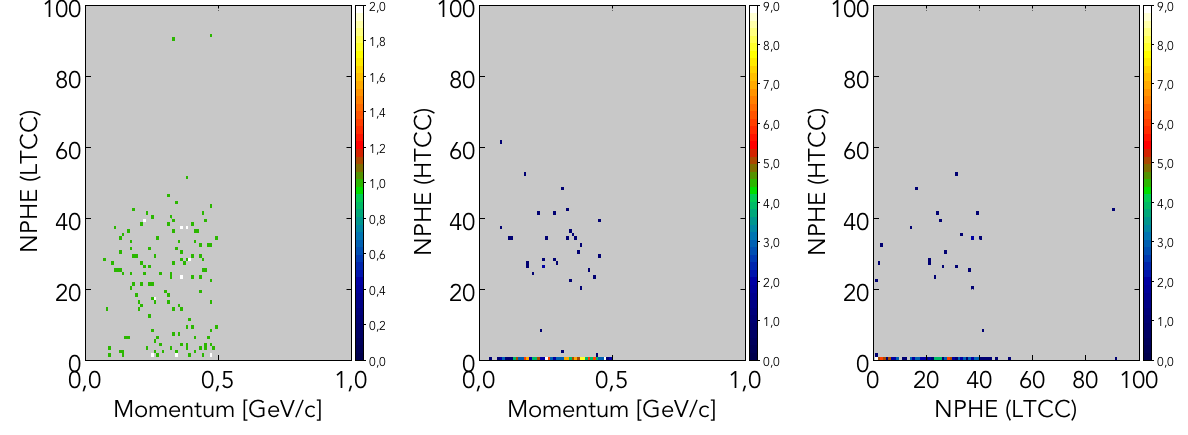
\includegraphics[width=1\textwidth,height=0.25\textwidth]{triggerStudies_Tor1_cut05_LTCC_HTCC_P_IN.png}\\
             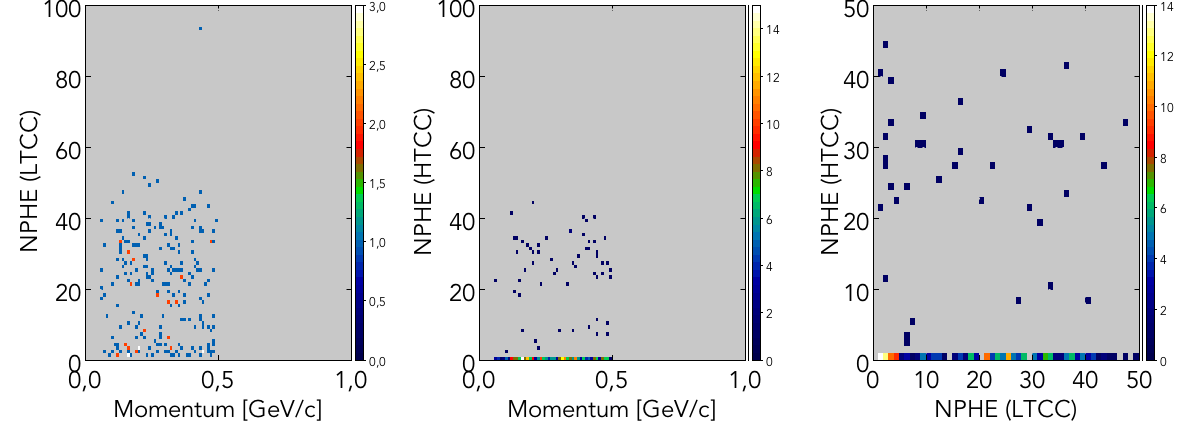
\includegraphics[width=1\textwidth,height=0.25\textwidth]{triggerStudies_Tor075_cut05_LTCC_HTCC_P_IN.png}
           \end{figure}
           
           Top: Torus: $-100\%$ / Bottom: Torus: $-75\%$
\end{frame}

\begin{frame}
	        \frametitle{LTCC and HTCC vs. Momentum}
	        \footnotesize
           \framesubtitle{$p(e^+)$ OR $p(e^-)$ $\le 0.5\,\rm{GeV/c}$}
           
           \begin{figure}
             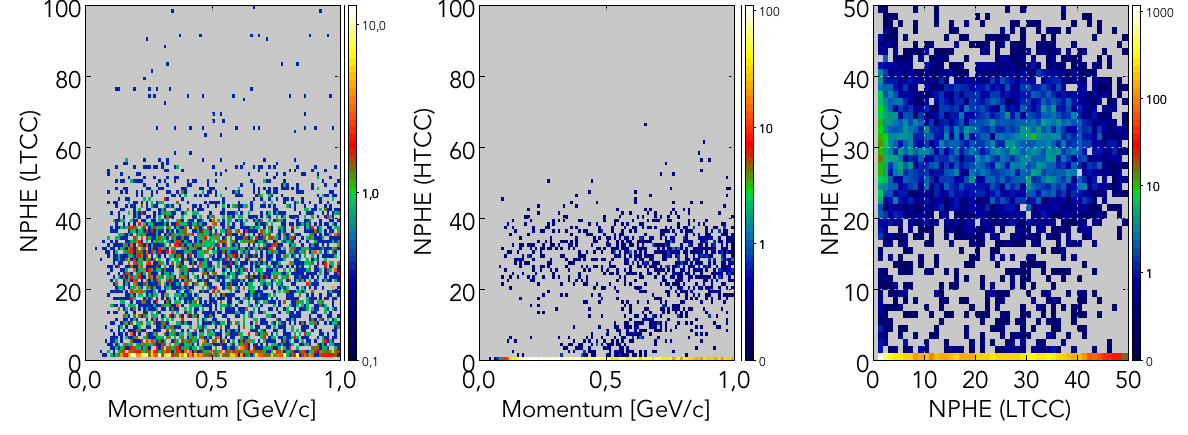
\includegraphics[width=1\textwidth,height=0.25\textwidth]{triggerStudies_Tor1_cut05_LTCC_HTCC_P_OUT.png}\\
             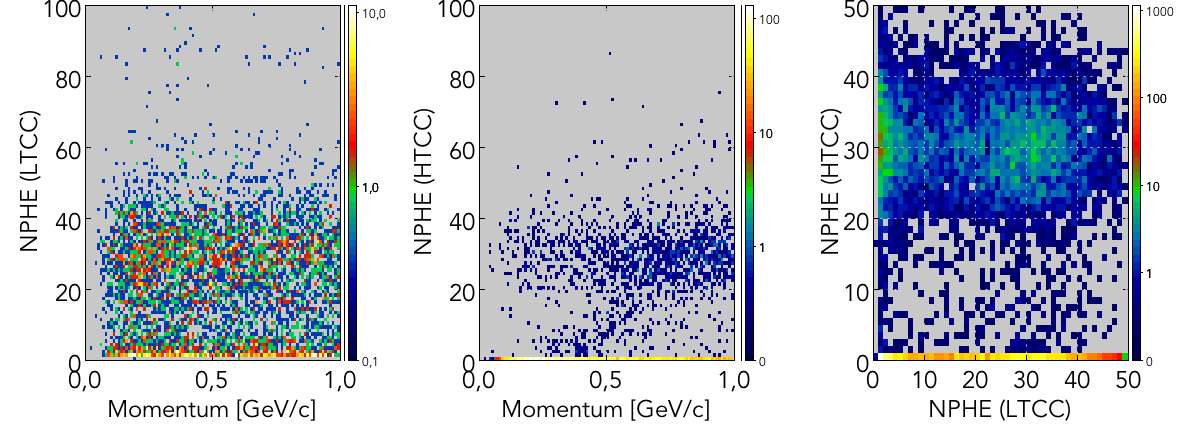
\includegraphics[width=1\textwidth,height=0.25\textwidth]{triggerStudies_Tor075_cut05_LTCC_HTCC_P_OUT.png}
           \end{figure}
           
           Top: Torus: $-100\%$ / Bottom: Torus: $-75\%$
\end{frame}

\begin{frame}
	        \frametitle{LTCC and HTCC vs. Momentum}
	        \footnotesize
           \framesubtitle{$p(e^+)$ AND $p(e^-)$ $\le 0.7\,\rm{GeV/c}$}
           
           \begin{figure}
             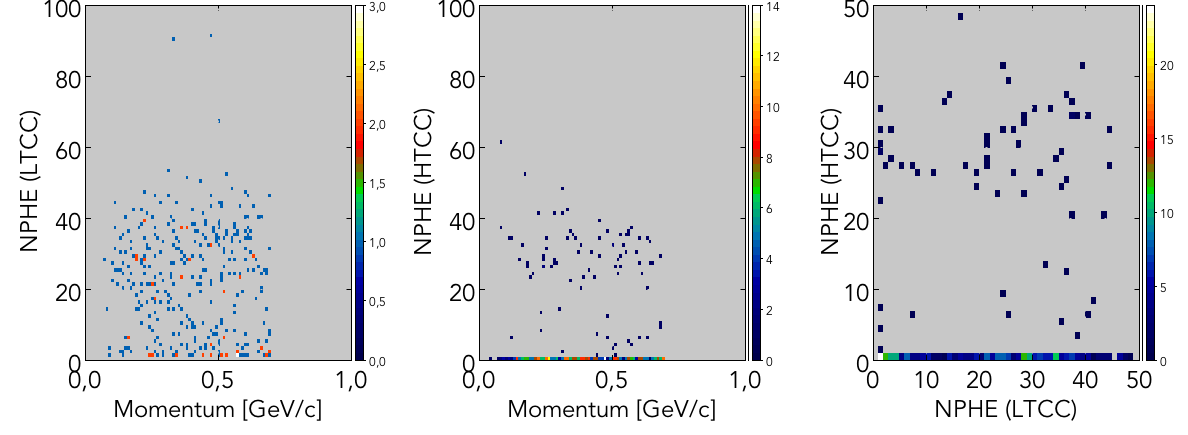
\includegraphics[width=1\textwidth,height=0.25\textwidth]{triggerStudies_Tor1_cut07_LTCC_HTCC_P_IN.png}\\
             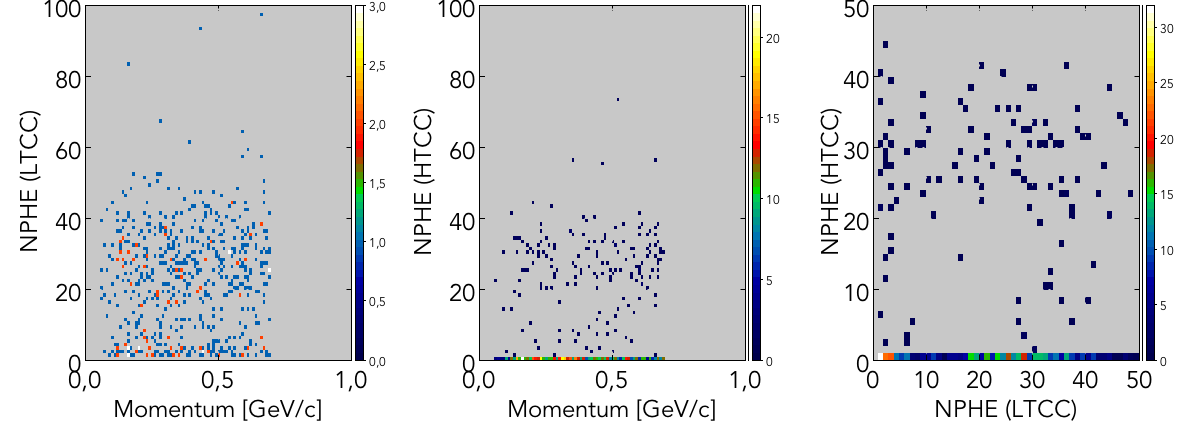
\includegraphics[width=1\textwidth,height=0.25\textwidth]{triggerStudies_Tor075_cut07_LTCC_HTCC_P_IN.png}
           \end{figure}
           
           Top: Torus: $-100\%$ / Bottom: Torus: $-75\%$
\end{frame}

\begin{frame}
	        \frametitle{LTCC and HTCC vs. Momentum}
	        \footnotesize
           \framesubtitle{$p(e^+)$ OR $p(e^-)$ $\le 0.7\,\rm{GeV/c}$}
           
           \begin{figure}
             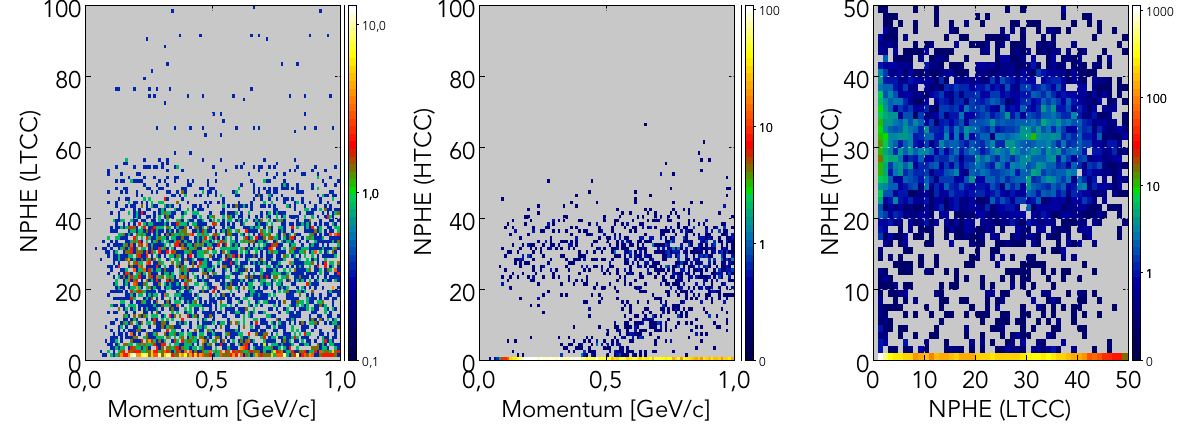
\includegraphics[width=1\textwidth,height=0.25\textwidth]{triggerStudies_Tor1_cut07_LTCC_HTCC_P_OUT.png}\\
             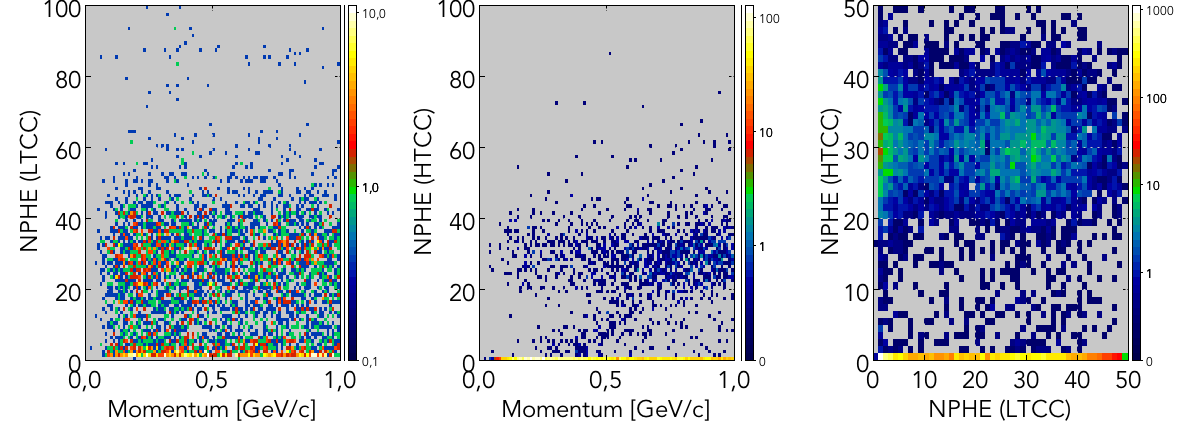
\includegraphics[width=1\textwidth,height=0.25\textwidth]{triggerStudies_Tor075_cut07_LTCC_HTCC_P_OUT.png}
           \end{figure}
           
           Top: Torus: $-100\%$ / Bottom: Torus: $-75\%$
      
      \end{frame}
      %***********************************************************************************************************
      
      
      %***********************************************************************************************************
      \begin{frame}
        \frametitle{$\Delta E(\text{PCAL + ECAL})$ vs. Momentum}
        \footnotesize
        \begin{figure}
          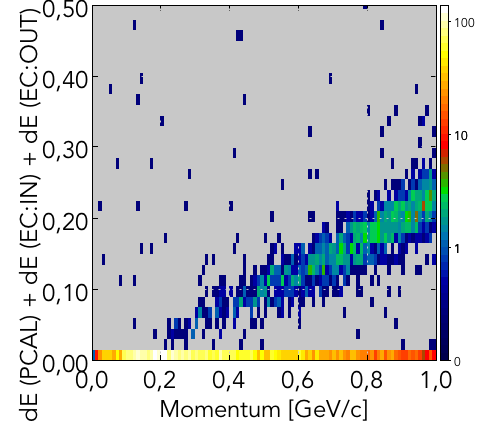
\includegraphics[width=0.25\textwidth,origin=l]{triggerStudies_Tor1_CAL.png}
          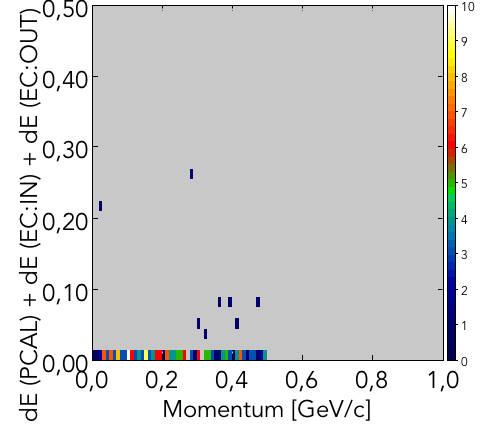
\includegraphics[width=0.25\textwidth]{triggerStudies_Tor1_cut05_CAL_IN.png}
          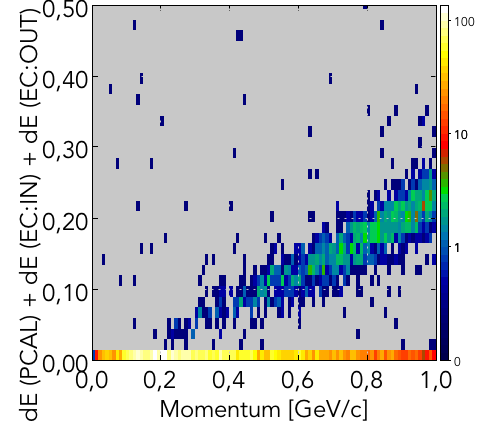
\includegraphics[width=0.25\textwidth,origin=r]{triggerStudies_Tor1_cut05_CAL_OUT.png}\\
            
          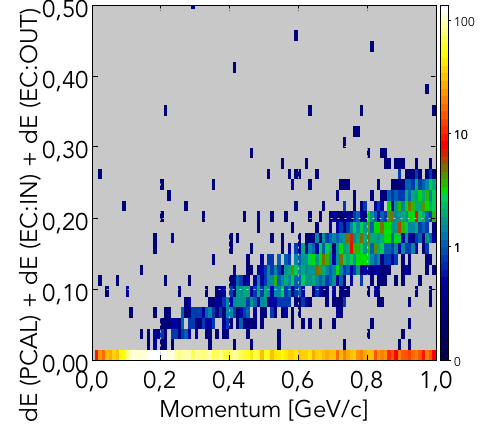
\includegraphics[width=0.25\textwidth,origin=l]{triggerStudies_Tor075_cut05_CAL.png}
          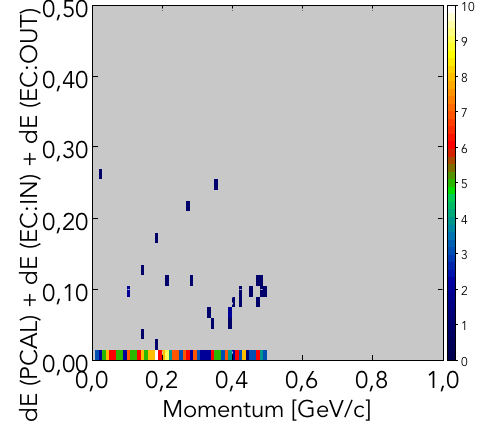
\includegraphics[width=0.25\textwidth]{triggerStudies_Tor075_cut05_CAL_IN.png}
           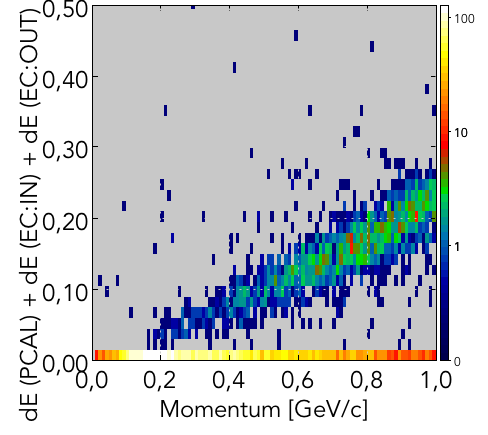
\includegraphics[width=0.25\textwidth,origin=r]{triggerStudies_Tor075_cut05_CAL_OUT.png}  
        \end{figure}
        
        \begin{itemize}
          \item Left: not cut 
          \item Centre: $p(e^+) \le 0.5\,\rm{GeV/c}$ and $p(e^-) \le 0.5\,\rm{GeV/c}$ 
          \item  Right: !($p(e^+) \le 0.5\,\rm{GeV/c}$ and $p(e^-) \le 0.5\,\rm{GeV/c}$)
          \item Top: Torus: $-100\%$ / Bottom: $-75\%$
        \end{itemize}
 \end{frame}
    
\begin{frame}
        \begin{figure}
          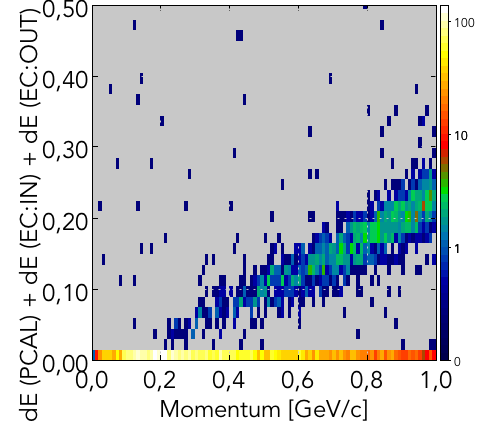
\includegraphics[width=0.25\textwidth,origin=l]{triggerStudies_Tor1_CAL.png}
          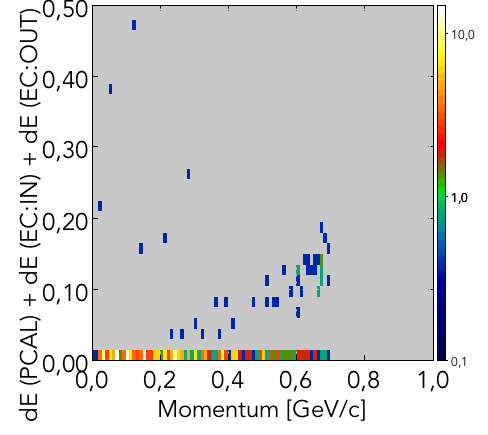
\includegraphics[width=0.25\textwidth]{triggerStudies_Tor1_cut07_CAL_IN.png}
          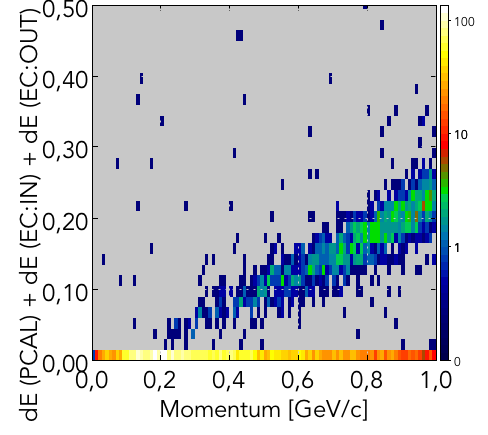
\includegraphics[width=0.25\textwidth,origin=r]{triggerStudies_Tor1_cut07_CAL_OUT.png}\\
            
          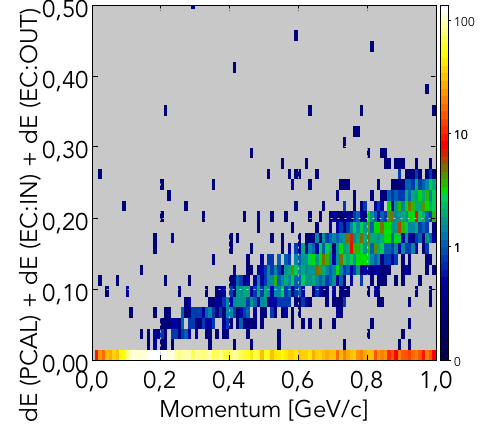
\includegraphics[width=0.25\textwidth,origin=l]{triggerStudies_Tor075_CAL.png}
          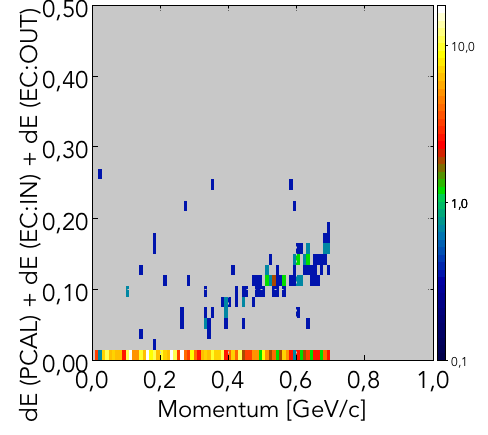
\includegraphics[width=0.25\textwidth]{triggerStudies_Tor075_cut07_CAL_IN.png}
           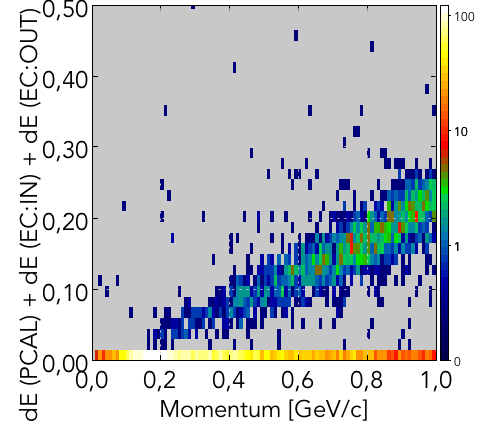
\includegraphics[width=0.25\textwidth,origin=r]{triggerStudies_Tor075_cut07_CAL_OUT.png}  
        \end{figure}
        
        \begin{itemize}
          \item Left: not cut 
          \item Centre: $p(e^+) \le 0.7\,\rm{GeV/c}$ and $p(e^-) \le 0.7\,\rm{GeV/c}$ 
          \item  Right: !($p(e^+) \le 0.7\,\rm{GeV/c}$ and $p(e^-) \le 0.7\,\rm{GeV/c}$)
          \item Top: Torus: $-100\%$ / Bottom: $-75\%$
        \end{itemize}       
\end{frame}

\begin{frame}
        \frametitle{Summary}

        \tiny
        \begin{table}
          \begin{tabular}{|c||c||c||c||c|}
             \hline
               Torus $[\%]$ & Cut: &  Momentum Range & $[\%]$ inside cut  & $[\%]$ outside cut \\
               \hline
               \hline
               $-100$ & $p(e^+)$ $\&$ $p(e^-)$ $ \lesssim 0.5\,\rm{GeV/c}$ & $p(e^+),p(e^-) \in [0,5] \,\rm{GeV/c}$  & $1\%$ & $99\%$\\
               \hline
                $-100$ & $p(e^+)$ $\&$ $p(e^-)$ $ \lesssim 0.5\,\rm{GeV/c}$ & $p(e^+),p(e^-) \in [0,4] \,\rm{GeV/c}$  & $2\%$ & $98\%$\\
                \hline
                 $-100$ & $p(e^+)$ $\&$ $p(e^-)$ $ \lesssim 0.5\,\rm{GeV/c}$ & $p(e^+),p(e^-) \in [0,3] \,\rm{GeV/c}$  & $2\%$ & $98\%$\\
                \hline
               $-100$ & $p(e^+)$ $\&$ $p(e^-)$ $ \lesssim 0.5\,\rm{GeV/c}$ & $p(e^+),p(e^-) \in [0,2] \,\rm{GeV/c}$  & $4\%$ & $96\%$\\
                \hline
                \hline
               $-100$ & $p(e^+)$ $\&$ $p(e^-)$ $ \lesssim 0.7\,\rm{GeV/c}$ & $p(e^+),p(e^-) \in [0,5] \,\rm{GeV/c}$  & $2\%$ & $98\%$\\
               \hline
                $-100$ & $p(e^+)$ $\&$ $p(e^-)$ $ \lesssim 0.7\,\rm{GeV/c}$ & $p(e^+),p(e^-) \in [0,4] \,\rm{GeV/c}$  & $3\%$ & $97\%$\\
                \hline
                 $-100$ & $p(e^+)$ $\&$ $p(e^-)$ $ \lesssim 0.7\,\rm{GeV/c}$ & $p(e^+),p(e^-) \in [0,3] \,\rm{GeV/c}$  & $5\%$ & $95\%$\\
                \hline
               $-100$ & $p(e^+)$ $\&$ $p(e^-)$ $ \lesssim 0.7\,\rm{GeV/c}$ & $p(e^+),p(e^-) \in [0,2] \,\rm{GeV/c}$  & $8\%$ & $92\%$\\
               \hline
               \hline
          \end{tabular}
        \end{table}
        
        \begin{itemize}
          \item Percentage inside cut: $\frac{\# \text{Events inside the cut}}{\# \text{Events within Momentum Range}}$ $\equiv$ Percentage of rejected events
           \item Percentage outside cut: $\frac{\# \text{Events outside the cut}}{\# \text{Events within Momentum Range}}$ $\equiv$ Percentage of accepted events
        \end{itemize}
\end{frame}
              
\begin{frame}  
        \tiny
        \begin{table}
          \begin{tabular}{|c||c||c||c||c|}
             \hline
               Torus $[\%]$ & Cut: &  Momentum Range & $[\%]$ inside cut  & $[\%]$ outside cut \\
               \hline
               \hline
               $-75$ & $p(e^+)$ $\&$ $p(e^-)$ $ \lesssim 0.5\,\rm{GeV/c}$ & $p(e^+),p(e^-) \in [0,5] \,\rm{GeV/c}$  & $1\%$ & $99\%$\\
               \hline
                $-75$ & $p(e^+)$ $\&$ $p(e^-)$ $ \lesssim 0.5\,\rm{GeV/c}$ & $p(e^+),p(e^-) \in [0,4] \,\rm{GeV/c}$  & $2\%$ & $98\%$\\
                \hline
                 $-75$ & $p(e^+)$ $\&$ $p(e^-)$ $ \lesssim 0.5\,\rm{GeV/c}$ & $p(e^+),p(e^-) \in [0,3] \,\rm{GeV/c}$  & $3\%$ & $97\%$\\
                \hline
               $-75$ & $p(e^+)$ $\&$ $p(e^-)$ $ \lesssim 0.5\,\rm{GeV/c}$ & $p(e^+),p(e^-) \in [0,2] \,\rm{GeV/c}$  & $5\%$ & $95\%$\\
                \hline
                \hline
               $-75$ & $p(e^+)$ $\&$ $p(e^-)$ $ \lesssim 0.7\,\rm{GeV/c}$ & $p(e^+),p(e^-) \in [0,5] \,\rm{GeV/c}$  & $2\%$ & $98\%$\\
               \hline
                $-75$ & $p(e^+)$ $\&$ $p(e^-)$ $ \lesssim 0.7\,\rm{GeV/c}$ & $p(e^+),p(e^-) \in [0,4] \,\rm{GeV/c}$  & $5\%$ & $95\%$\\
                \hline
                 $-75$ & $p(e^+)$ $\&$ $p(e^-)$ $ \lesssim 0.7\,\rm{GeV/c}$ & $p(e^+),p(e^-) \in [0,3] \,\rm{GeV/c}$  & $7\%$ & $93\%$\\
                \hline
               $-75$ & $p(e^+)$ $\&$ $p(e^-)$ $ \lesssim 0.7\,\rm{GeV/c}$ & $p(e^+),p(e^-) \in [0,2] \,\rm{GeV/c}$  & $12\%$ & $88\%$\\
               \hline
               \hline
          \end{tabular}
        \end{table}  
		\begin{itemize}
	          \item Percentage inside cut: $\frac{\# \text{Events inside the cut}}{\# \text{Events within Momentum Range}}$ $\equiv$ Percentage of rejected events
			 \item Percentage outside cut: $\frac{\# \text{Events outside the cut}}{\# \text{Events within Momentum Range}}$ $\equiv$ Percentage of accepted events
	\end{itemize}        
\end{frame}
      %*********************************************************************************************************** 
\begin{frame}
	\frametitle{IKP Trigger Request for $\eta'$ Dalitz channel}
	\begin{itemize}
		\item HTCC NPE > 5
       	\item PCAL + EC sum > 150MeV

       	\item This would be a 12\% loss of signal for dilepton pairs that correspond to momentum of 0.7GeV/c each in the momentum range $0-2GeV/c$.
    \end{itemize}
\end{frame}
      
      
             
         
         
 \end{document}